\chapter{Analyse expérimentale de la sensibilité fréquentielle des CNN}

\section{Objectif et positionnement du chapitre}
\label{sec:objectif_positionnement_chapitre4}

Dans le chapitre précédent, nous avons montré que les fonctions de Fourier jouent un rôle particulier
dans l'analyse des opérateurs de convolution. Dans le cadre linéaire idéalisé, certaines directions
fréquentielles apparaissent comme des directions privilégiées de l'opérateur convolutionnel. Dans un
CNN réel, composé notamment de ReLU et de max-pooling, cette propriété n'est plus globale ni exacte,
mais elle peut encore être interprétée localement à travers le jacobien du modèle.

L'objectif de ce chapitre est donc de vérifier expérimentalement si cette sensibilité fréquentielle reste
observable dans un CNN entraîné sur des données réelles. Nous ne cherchons pas à reproduire l'ensemble
des expériences de Tsuzuku et Sato~\cite{tsuzuku2019structural}, mais à reprendre leur mécanisme
central : tester systématiquement des perturbations construites à partir de fréquences de Fourier et
mesurer leur capacité à modifier les prédictions du modèle.

Notre protocole se concentre sur une architecture de type VGG avec normalisation par batch,
notée \texttt{VGGSmallBN}, entraînée sur CIFAR-10 et CIFAR-100. Pour chaque fréquence $(u,v)$,
nous construisons une perturbation universelle de Fourier, puis nous mesurons la proportion de
prédictions modifiées. Cette mesure, appelée \textit{fool ratio}, permet de construire une carte de
sensibilité fréquentielle du modèle.

Notre reproduction est volontairement plus restreinte que celle de Tsuzuku et Sato, mais conserve les éléments essentiels : construction d'une perturbation de Fourier,
contrôle de son amplitude, calcul du \textit{fool ratio} et génération d'une heatmap fréquentielle.

L'amplitude principale est fixée à
\[
    \epsilon = 10/255,
\]
comme dans les expériences CIFAR de l'article original. Nous ajoutons ensuite deux contrôles
expérimentaux : une comparaison avec un bruit aléatoire de même amplitude et un balayage de
plusieurs valeurs de $\epsilon$.

Enfin, contrairement à l'algorithme de heatmap de l'article, qui évalue chaque fréquence sur un
minibatch, nous évaluons chaque fréquence sur l'ensemble de test complet. Ce choix rend le calcul
plus coûteux, mais fournit une estimation plus stable du \textit{fool ratio}. 

\section{Cadre expérimental retenu}

\subsection{Jeux de données}

Nous utilisons CIFAR-10 et CIFAR-100. Les deux jeux de données contiennent des images RGB de
taille $32\times32$, ce qui permet de conserver le même domaine fréquentiel dans les deux expériences :
\[
    (u,v) \in \{0,\dots,31\}^2.
\]

CIFAR-10 contient $10$ classes et constitue un premier cadre de reproduction relativement stable.
CIFAR-100 contient $100$ classes pour la même résolution d'image ; la tâche est donc plus difficile,
car les catégories sont plus nombreuses et souvent visuellement proches. La comparaison entre les
deux permet d'observer si la sensibilité fréquentielle persiste lorsque la classification devient plus fine.

\subsection{Architecture étudiée}

Pour cette reproduction expérimentale, nous utilisons une architecture convolutionnelle de type VGG
avec normalisation par batch, que nous appelons \texttt{VGGSmallBN}. L'objectif n'est pas de reproduire
exactement une architecture VGG historique~\cite{simonyan2015very}, mais de conserver son principe
général : empiler plusieurs blocs convolutionnels simples, composés de convolutions $3\times3$,
de normalisations par batch, d'activations ReLU et de couches de réduction spatiale.

Le réseau est composé de quatre blocs convolutionnels. Chaque bloc contient deux convolutions
$3\times3$, chacune suivie d'une normalisation par batch et d'une activation ReLU. Le bloc se termine
par un \textit{max pooling} $2\times2$, qui divise par deux la résolution spatiale. La tête de
classification applique ensuite un \textit{adaptive average pooling}, aplatit le tenseur obtenu, puis
utilise une couche linéaire finale. Cette architecture est résumée dans la figure~\ref{fig:vgg_small_bn_v3}.

\begin{figure}[H]
    \centering
    \resizebox{\textwidth}{!}{
    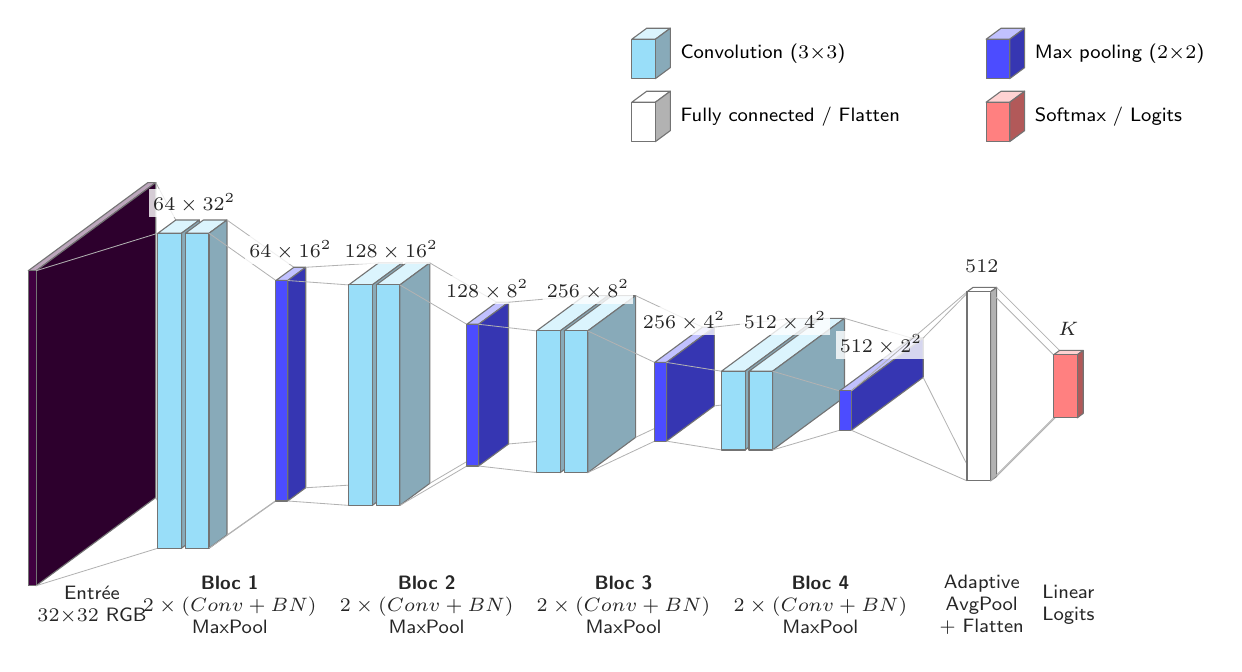
\begin{tikzpicture}[
        x={(1cm,0cm)},
        y={(0cm,1cm)},
        z={(0.38cm,0.28cm)},
        font=\sffamily\footnotesize,
        dimlabel/.style={
            align=center,
            text=black!85,
            font=\sffamily\scriptsize,
            fill=white,
            fill opacity=0.8,
            text opacity=1,
            inner sep=1.5pt
        },
        blocklabel/.style={
            align=center,
            text=black!85,
            font=\sffamily\scriptsize
        }
    ]

    % --- Définition des couleurs ---
    \colorlet{colIn}{violet!50!black}
    \colorlet{colConv}{cyan!40}
    \colorlet{colPool}{blue!70}
    \colorlet{colFC}{white}
    \colorlet{colSoftmax}{red!50}

    % --- Macros de dessin ---
    \def\drawbox#1#2#3#4#5{
        \pgfmathsetmacro{\yy}{-#2/2}
        \pgfmathsetmacro{\zz}{-#3/2}
        \filldraw[fill=#5!35!white, draw=black!55, line width=0.4pt, line join=round]
            (#1,\yy+#2,\zz) -- (#1+#4,\yy+#2,\zz) -- (#1+#4,\yy+#2,\zz+#3) -- (#1,\yy+#2,\zz+#3) -- cycle;
        \filldraw[fill=#5!70!black, draw=black!55, line width=0.4pt, line join=round]
            (#1+#4,\yy,\zz) -- (#1+#4,\yy,\zz+#3) -- (#1+#4,\yy+#2,\zz+#3) -- (#1+#4,\yy+#2,\zz) -- cycle;
        \filldraw[fill=#5, draw=black!55, line width=0.4pt, line join=round]
            (#1,\yy,\zz) -- (#1+#4,\yy,\zz) -- (#1+#4,\yy+#2,\zz) -- (#1,\yy+#2,\zz) -- cycle;
    }

    \def\connect#1#2#3#4#5#6{
        \draw[black!30, line width=0.3pt, line join=round] (#1, #2/2, -#3/2) -- (#4, #5/2, -#6/2);
        \draw[black!30, line width=0.3pt, line join=round] (#1, -#2/2, -#3/2) -- (#4, -#5/2, -#6/2);
        \draw[black!30, line width=0.3pt, line join=round] (#1, #2/2, #3/2) -- (#4, #5/2, #6/2);
        \draw[black!30, line width=0.3pt, line join=round] (#1, -#2/2, #3/2) -- (#4, -#5/2, #6/2);
    }

    % ==================================================================
    % ARCHITECTURE DU RESEAU
    % ==================================================================

    % --- Entrée (Rendu comme une image carrée 32x32) ---
    \drawbox{0.0}{4.0}{4.0}{0.1}{colIn} % Hauteur 4, Profondeur 4 = Carré
    \node[blocklabel] at (0.05, -2.8, 0) {Entrée\\$32{\times}32$ RGB};
    \connect{0.1}{4.0}{4.0}{1.0}{4.0}{0.6}

    % --- Bloc 1 (avec micro-espace entre Conv) ---
    \drawbox{1.0}{4.0}{0.6}{0.3}{colConv} % Conv 1
    \drawbox{1.35}{4.0}{0.6}{0.3}{colConv} % Conv 2 (Ecart de 0.05)
    \node[dimlabel] at (1.35, 2.3, 0) {$64 \times 32^2$};
    
    \connect{1.65}{4.0}{0.6}{2.5}{2.8}{0.6}
    \drawbox{2.5}{2.8}{0.6}{0.15}{colPool}
    \node[dimlabel] at (2.57, 1.7, 0) {$64 \times 16^2$};
    
    \node[blocklabel] at (1.8, -2.8, 0) {\textbf{Bloc 1}\\$2\times(\text{Conv}+\text{BN})$\\MaxPool};
    \connect{2.65}{2.8}{0.6}{3.5}{2.8}{1.0}

    % --- Bloc 2 ---
    \drawbox{3.5}{2.8}{1.0}{0.3}{colConv}
    \drawbox{3.85}{2.8}{1.0}{0.3}{colConv}
    \node[dimlabel] at (3.85, 1.7, 0) {$128 \times 16^2$};

    \connect{4.15}{2.8}{1.0}{5.0}{1.8}{1.0}
    \drawbox{5.0}{1.8}{1.0}{0.15}{colPool}
    \node[dimlabel] at (5.07, 1.2, 0) {$128 \times 8^2$};

    \node[blocklabel] at (4.3, -2.8, 0) {\textbf{Bloc 2}\\$2\times(\text{Conv}+\text{BN})$\\MaxPool};
    \connect{5.15}{1.8}{1.0}{6.0}{1.8}{1.6}

    % --- Bloc 3 ---
    \drawbox{6.0}{1.8}{1.6}{0.3}{colConv}
    \drawbox{6.35}{1.8}{1.6}{0.3}{colConv}
    \node[dimlabel] at (6.35, 1.2, 0) {$256 \times 8^2$};

    \connect{6.65}{1.8}{1.6}{7.5}{1.0}{1.6}
    \drawbox{7.5}{1.0}{1.6}{0.15}{colPool}
    \node[dimlabel] at (7.57, 0.8, 0) {$256 \times 4^2$};

    \node[blocklabel] at (6.8, -2.8, 0) {\textbf{Bloc 3}\\$2\times(\text{Conv}+\text{BN})$\\MaxPool};
    \connect{7.65}{1.0}{1.6}{8.5}{1.0}{2.4}

    % --- Bloc 4 ---
    \drawbox{8.5}{1.0}{2.4}{0.3}{colConv}
    \drawbox{8.85}{1.0}{2.4}{0.3}{colConv}
    \node[dimlabel] at (8.85, 0.8, 0) {$512 \times 4^2$};

    \connect{9.15}{1.0}{2.4}{10.0}{0.5}{2.4}
    \drawbox{10.0}{0.5}{2.4}{0.15}{colPool}
    \node[dimlabel] at (10.07, 0.5, 0) {$512 \times 2^2$};

    \node[blocklabel] at (9.3, -2.8, 0) {\textbf{Bloc 4}\\$2\times(\text{Conv}+\text{BN})$\\MaxPool};
    \connect{10.15}{0.5}{2.4}{11.2}{2.4}{0.2}

    % --- Tête finale ---
    \drawbox{11.2}{2.4}{0.2}{0.3}{colFC}
    \node[dimlabel] at (11.35, 1.5, 0) {$512$};
    \node[blocklabel] at (11.35, -2.8, 0) {Adaptive\\AvgPool\\+ Flatten};
    \connect{11.5}{2.4}{0.2}{12.3}{0.8}{0.2}

    \drawbox{12.3}{0.8}{0.2}{0.3}{colSoftmax}
    \node[dimlabel] at (12.45, 0.7, 0) {$K$};
    \node[blocklabel] at (12.45, -2.8, 0) {Linear\\Logits};

    % --- Légende ---
    \begin{scope}[shift={(7.0, 4.2)}] 
        \begin{scope}[shift={(0, 0)}]
            \drawbox{0}{0.5}{0.5}{0.3}{colConv}
            \node[right, font=\sffamily\scriptsize] at (0.4, 0, 0) {Convolution ($3{\times}3$)};
        \end{scope}
        \begin{scope}[shift={(0, -0.8)}]
            \drawbox{0}{0.5}{0.5}{0.3}{colFC}
            \node[right, font=\sffamily\scriptsize] at (0.4, 0, 0) {Fully connected / Flatten};
        \end{scope}
        \begin{scope}[shift={(4.5, 0)}]
            \drawbox{0}{0.5}{0.5}{0.3}{colPool}
            \node[right, font=\sffamily\scriptsize] at (0.4, 0, 0) {Max pooling ($2{\times}2$)};
        \end{scope}
        \begin{scope}[shift={(4.5, -0.8)}]
            \drawbox{0}{0.5}{0.5}{0.3}{colSoftmax}
            \node[right, font=\sffamily\scriptsize] at (0.4, 0, 0) {Softmax / Logits};
        \end{scope}
    \end{scope}

    \end{tikzpicture}
    }
    \caption{Illustration de l'architecture \texttt{VGGSmallBN} utilise, où $K$ désigne le nombre de classes du dataset : $K=10$ pour CIFAR-10 et $K=100$ pour CIFAR-100.}
    \label{fig:vgg_small_bn_v3}
\end{figure}

\subsection{Paramètres d'entraînement}

\begin{table}[H]
    \centering
    \small
    \begin{tabular}{|l|l|}
        \hline
        \textbf{Paramètre} & \textbf{Valeur retenue} \\
        \hline
        Nombre d'époques & $100$ \\
        \hline
        Optimiseur & SGD \\
        \hline
        Taux d'apprentissage initial & $0.1$ \\
        \hline
        Momentum & $0.9$ \\
        \hline
        Weight decay & $5\cdot 10^{-4}$ \\
        \hline
        Scheduler & Cosine annealing \\
        \hline
        Taille de batch & $256$ \\
        \hline
        Jeux de données & CIFAR-10 et CIFAR-100 \\
        \hline
        Architecture & \texttt{VGGSmallBN} \\
        \hline
    \end{tabular}
    \caption{Paramètres d'entraînement utilisés pour les modèles \texttt{VGGSmallBN}.}
    \label{tab:parametres_entrainement_vgg}
\end{table}

Le momentum permet de stabiliser les mises à jour des poids et
d'accélérer l'optimisation. Le \textit{weight decay} joue un rôle de régularisation : il pénalise les poids
trop grands et limite ainsi le risque de surapprentissage.

Le taux d'apprentissage initial est fixé à $0.1$, puis diminué progressivement à l'aide d'un scheduler
de type \textit{cosine annealing}. L'idée est de laisser le modèle apprendre rapidement au début de
l'entraînement, puis d'effectuer des ajustements plus fins lorsque l'on se rapproche de la fin. Enfin,
nous entraînons le modèle pendant $100$ époques avec une taille de batch de $256$, ce qui permet
d'exploiter efficacement le GPU disponible tout en conservant un entraînement stable.

\subsection{Performance de référence}

\begin{table}[H]
    \centering
    \small
    \begin{tabular}{|l|c|c|c|}
        \hline
        \textbf{Dataset} & \textbf{Nombre de classes} & \textbf{Validation} & \textbf{Test} \\
        \hline
        CIFAR-10 & $10$ & $93.86\,\%$ & $93.07\,\%$ \\
        \hline
        CIFAR-100 & $100$ & $73.04\,\%$ & $72.55\,\%$ \\
        \hline
    \end{tabular}
    \caption{Performances de référence des modèles \texttt{VGGSmallBN} avant ajout de perturbations.}
    \label{tab:performance_reference_vgg}
\end{table}

La différence entre les deux datasets est attendue : CIFAR-100 contient dix fois plus de classes que
CIFAR-10, avec des catégories souvent plus proches visuellement. Dans les deux cas, les performances
sont suffisamment élevées pour que l'étude des perturbations soit interprétable : les modèles ne sont
pas parfaits, mais ils constituent des classifieurs de référence crédibles.

\section{Construction des perturbations de Fourier}
\label{sec:construction_perturbations_fourier}

L'idée générale est de construire une perturbation universelle. Contrairement à une attaque adversariale classique, 
la perturbation n'est pas optimisée séparément pour chaque image. 
Elle dépend uniquement d'une fréquence $(u,v)$ et d'une amplitude $\epsilon$. 
On cherche ensuite à savoir si cette direction fréquentielle, bien qu'elle ne soit pas un vecteur propre
global du réseau réel, suffit à modifier les prédictions du modèle sur un grand nombre d'images.

\subsection{Single Fourier Attack}
\label{subsec:single_fourier_attack}

La \textit{Single Fourier Attack} (SFA) proposée par Tsuzuku et Sato~\cite{tsuzuku2019structural}
consiste à construire une perturbation à partir d'une seule fréquence de Fourier. L'idée principale
est simple : au lieu d'optimiser une perturbation différente pour chaque image, on choisit une
fréquence $(u,v)$, on construit le motif spatial correspondant, puis on ajoute ce même motif à toutes
les images.

Dans notre protocole, une fréquence est représentée par un couple
\[
    (u,v) \in \{0,\dots,N-1\}^2,
\]
où $N$ désigne la taille spatiale de l'image. 

Pour une fréquence donnée $(u,v)$, on note $\delta_{u,v}$ la perturbation construite à partir de cette
fréquence. L'image perturbée est alors définie par
\begin{equation}
    \tilde{x}_{i}
    =
    \operatorname{clip}_{[0,1]}\left(x_i + \delta_{u,v,i}\right)
    =
    \begin{cases}
        0, & \text{si } x_i + \delta_{u,v,i} < 0, \\
        x_i + \delta_{u,v,i}, & \text{si } x_i + \delta_{u,v,i} \in [0,1], \\
        1, & \text{si } x_i + \delta_{u,v,i} > 1.
    \end{cases}
    \label{eq:single_fourier_attack}
\end{equation}
où $x$ est l'image initiale, $\tilde{x}$ l'image perturbée, et où le clipping garantit que les valeurs de
pixels restent dans l'intervalle valide $[0,1]$.

En pratique, pour chaque fréquence $(u,v)$, nous construisons d'abord un motif spatial réel
$p_{u,v}$. Ce motif est ensuite normalisé en norme $\ell_\infty$, afin que son amplitude maximale
soit égale à l'amplitude choisie $\epsilon$ :
\begin{equation}
    \delta_{u,v}
    =
    \epsilon
    \frac{p_{u,v}}{\|p_{u,v}\|_\infty}.
    \label{eq:normalisation_sfa}
\end{equation}

Ainsi, si une fréquence obtient un \textit{fool ratio} plus élevé qu'une autre,
ce n'est pas parce qu'elle a été testée avec une perturbation plus grande, mais parce que sa direction
fréquentielle perturbe davantage le modèle.

Pour les images RGB de CIFAR-10 et CIFAR-100, le même motif spatial est appliqué aux trois canaux
couleur.
La perturbation finale possède donc la même structure fréquentielle dans chaque canal. Après ajout
de la perturbation, l'image est ramenée dans l'intervalle $[0,1]$, normalisée avec les statistiques du dataset considéré 
avant d'être donnée au modèle.

L'algorithme~\ref{algo:single_fourier_attack} résume la procédure utilisée dans notre implémentation.

\begin{algorithm}[H]
\caption{Single Fourier Attack utilisée dans notre protocole}
\label{algo:single_fourier_attack}
\begin{algorithmic}
\State \textbf{input} : image $x$, fréquence $(u,v)$, amplitude $\epsilon$
\State \textbf{output} : image perturbée $\tilde{x}$
\State
\State Construire le motif spatial réel $p_{u,v}$
\State Normaliser ce motif en norme $\ell_\infty$ :
\State \hspace{0.5cm} $\delta_{u,v} \leftarrow \epsilon \dfrac{p_{u,v}}{\|p_{u,v}\|_\infty}$
\State Ajouter la perturbation à l'image :
\State \hspace{0.5cm} $x_{\mathrm{pert}} \leftarrow x + \delta_{u,v}$
\State Appliquer le clipping :
\State \hspace{0.5cm} $\tilde{x} \leftarrow \operatorname{clip}_{[0,1]}(x_{\mathrm{pert}})$
\State \Return $\tilde{x}$
\end{algorithmic}
\end{algorithm}

\subsection{Contrôle de l'amplitude}

Dans notre protocole principal, nous utilisons la même borne que celle utilisée dans l'article original
pour CIFAR :
\[
    \epsilon = \frac{10}{255}.
\]
Cette valeur signifie que chaque pixel peut être modifié d'au plus $10$ niveaux sur une échelle de
$0$ à $255$.

Pour chaque fréquence $(u,v)$, la perturbation est normalisée de manière à vérifier
\[
    \|\delta_{u,v}\|_{\infty} \leq \epsilon.
\]

Après ajout de la perturbation, l'image est ramenée dans l'intervalle valide $[0,1]$ par clipping, comme
dans l'équation~\eqref{eq:single_fourier_attack}.

La figure~\ref{fig:sfa_spatial_pattern_vgg_cifar10} montre, à titre d'exemple, le motif spatial obtenu
pour la fréquence $(16,24)$, qui correspond à la meilleure direction trouvée sur CIFAR-10.

\begin{figure}[H]
    \centering
    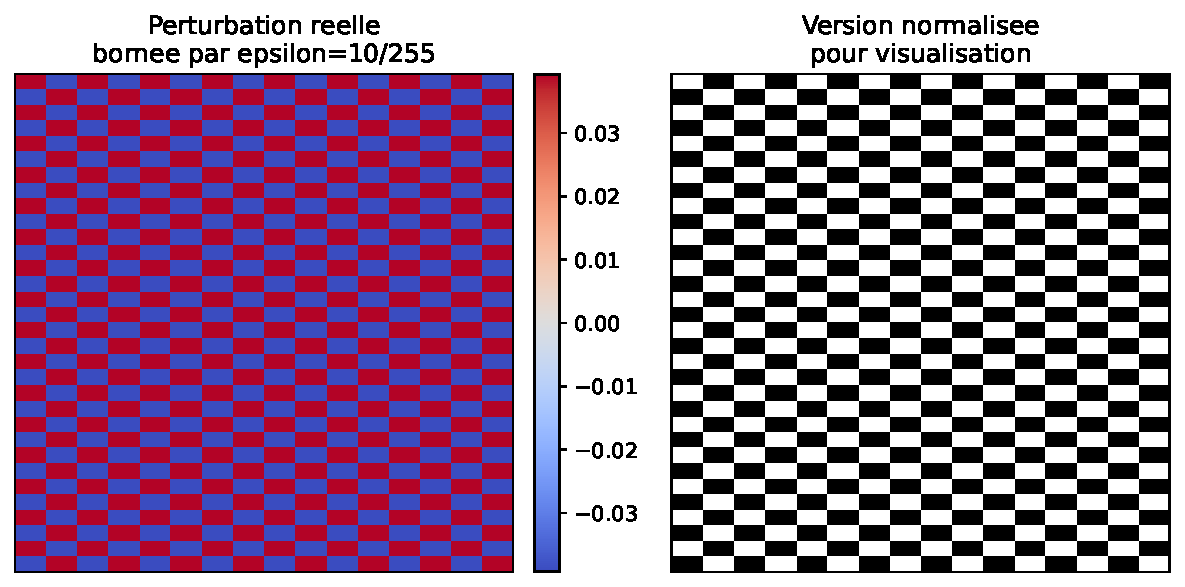
\includegraphics[width=0.55\textwidth]{figures/results/sfa_spatial_pattern_vgg_cifar10.pdf}
    \caption{Motif spatial associé à la perturbation SFA pour la fréquence $(16,24)$. La visualisation est
    normalisée afin de rendre la structure du motif visible.}
    \label{fig:sfa_spatial_pattern_vgg_cifar10}
\end{figure}

\section{Mesure de la sensibilité fréquentielle}
\label{sec:mesure_sensibilite_frequentielle}

Une fois les perturbations de Fourier définies, il faut mesurer leur effet sur le modèle.

\subsection{Définition du fool ratio}
\label{subsec:def_fool_ratio}

Soit $f$ le modèle étudié, et soit $\mathcal{D}=\{x_1,\dots,x_M\}$ un ensemble d'images. Pour une
fréquence $(u,v)$ donnée, on note $\tilde{x}_k^{(u,v)}$ l'image obtenue en ajoutant à $x_k$ la perturbation
de Fourier associée à cette fréquence.

Le \textit{fool ratio} mesure la proportion d'images pour lesquelles la prédiction du modèle change
après perturbation :
\[
    \operatorname{FR}(u,v)
    =
    \frac{1}{M}
    \sum_{k=1}^{M}
    \mathbf{1}
    \left[
        f(x_k) \neq f\!\left(\tilde{x}_k^{(u,v)}\right)
    \right].
\]

Cette mesure ne compare pas directement la prédiction au label réel. Elle compare uniquement la
prédiction du modèle avant et après perturbation. Ainsi, une image est comptée comme réussie pour
l'attaque lorsque la perturbation modifie la décision du modèle.

Le \textit{fool ratio} indique donc dans quelle mesure une direction fréquentielle est capable de modifier
les prédictions, indépendamment de la classe réelle des images.

% \subsection{Stabilité entre heatmaps}

% Pour comparer les heatmaps obtenues avec différentes seeds d'entraînement, nous utilisons deux
% mesures de corrélation. Chaque heatmap est d'abord aplatie en un vecteur de taille $32\times32$,
% contenant les \textit{fool ratios} de toutes les fréquences.

% La corrélation de Pearson mesure si deux heatmaps ont une structure globale similaire en valeur. La
% corrélation de Spearman compare plutôt l'ordre relatif des fréquences, en remplaçant les valeurs par
% leurs rangs. Elle permet donc de vérifier si les fréquences les plus sensibles restent globalement les
% mêmes d'un entraînement à l'autre, même lorsque les valeurs exactes des \textit{fool ratios} changent
% légèrement.

\subsection{Génération des heatmaps}
\label{subsec:generation_heatmaps}

Une heatmap de sensibilité fréquentielle est une matrice $H \in \mathbb{R}^{32\times32}$ dont chaque
case correspond à une fréquence $(u,v)$. La valeur $H_{u,v}$ est le \textit{fool ratio} obtenu lorsque
la perturbation de Fourier associée à cette fréquence est ajoutée aux images de test.

Le calcul suit trois étapes : d'abord, nous calculons les prédictions du modèle sur les images propres ;
ensuite, pour chaque fréquence, nous appliquons la perturbation correspondante ; enfin, nous mesurons
la proportion de prédictions modifiées. Cette procédure est résumée dans
l'algorithme~\ref{algo:algorithme_heatmap}.

\begin{algorithm}[H]
\caption{Génération d'une heatmap de sensibilité fréquentielle}
\label{algo:algorithme_heatmap}
\begin{algorithmic}
\State \textbf{input} : modèle $f$, images de test $\mathcal{D}$, amplitude $\epsilon$
\State \textbf{output} : heatmap $H \in \mathbb{R}^{32 \times 32}$
\State
\State $y \leftarrow f(\mathcal{D})$ \Comment{prédictions sur les images propres}
\For{$u = 0$ \textbf{to} $31$}
    \For{$v = 0$ \textbf{to} $31$}
        \State $\delta_{u,v} \leftarrow$ construire la perturbation de Fourier de fréquence $(u,v)$
        \State $\tilde{\mathcal{D}}_{u,v} \leftarrow \operatorname{clip}_{[0,1]}(\mathcal{D} + \delta_{u,v})$
        \State $\tilde{y}_{u,v} \leftarrow f(\tilde{\mathcal{D}}_{u,v})$
        \State $H_{u,v} \leftarrow \operatorname{FoolRatio}(y,\tilde{y}_{u,v})$
    \EndFor
\EndFor
\end{algorithmic}
\end{algorithm}

\subsection{Choix de la fréquence la plus sensible}
\label{subsec:choix_frequence_sensible}

Une fois la heatmap calculée, nous sélectionnons la fréquence qui maximise le \textit{fool ratio} :
\[
    (u^\star,v^\star)
    =
    \arg\max_{(u,v)}
    \operatorname{FR}(u,v).
\]

Cette fréquence correspond à la perturbation de Fourier la plus efficace parmi toutes celles testées
dans le protocole.

Cette sélection est effectuée séparément pour CIFAR-10 et CIFAR-100. Les fréquences obtenues et
leur interprétation sont présentées dans la section~\ref{subsec:frequences_plus_sensibles}.

\section{Résultats expérimentaux}
\label{sec:resultats_experimentaux}

\subsection{Heatmaps de sensibilité fréquentielle}
\label{subsec:resultats_heatmaps}

La méthodologie décrite précédemment nous permet de construire les cartes de sensibilité fréquentielle
du modèle \texttt{VGGSmallBN}. La figure~\ref{fig:heatmap_comparison_vgg_cifar10_cifar100}
compare les résultats obtenus sur nos deux datasets pour une même amplitude de perturbation,
fixée à $\epsilon = 10/255$.

\begin{figure}[H]
    \centering
    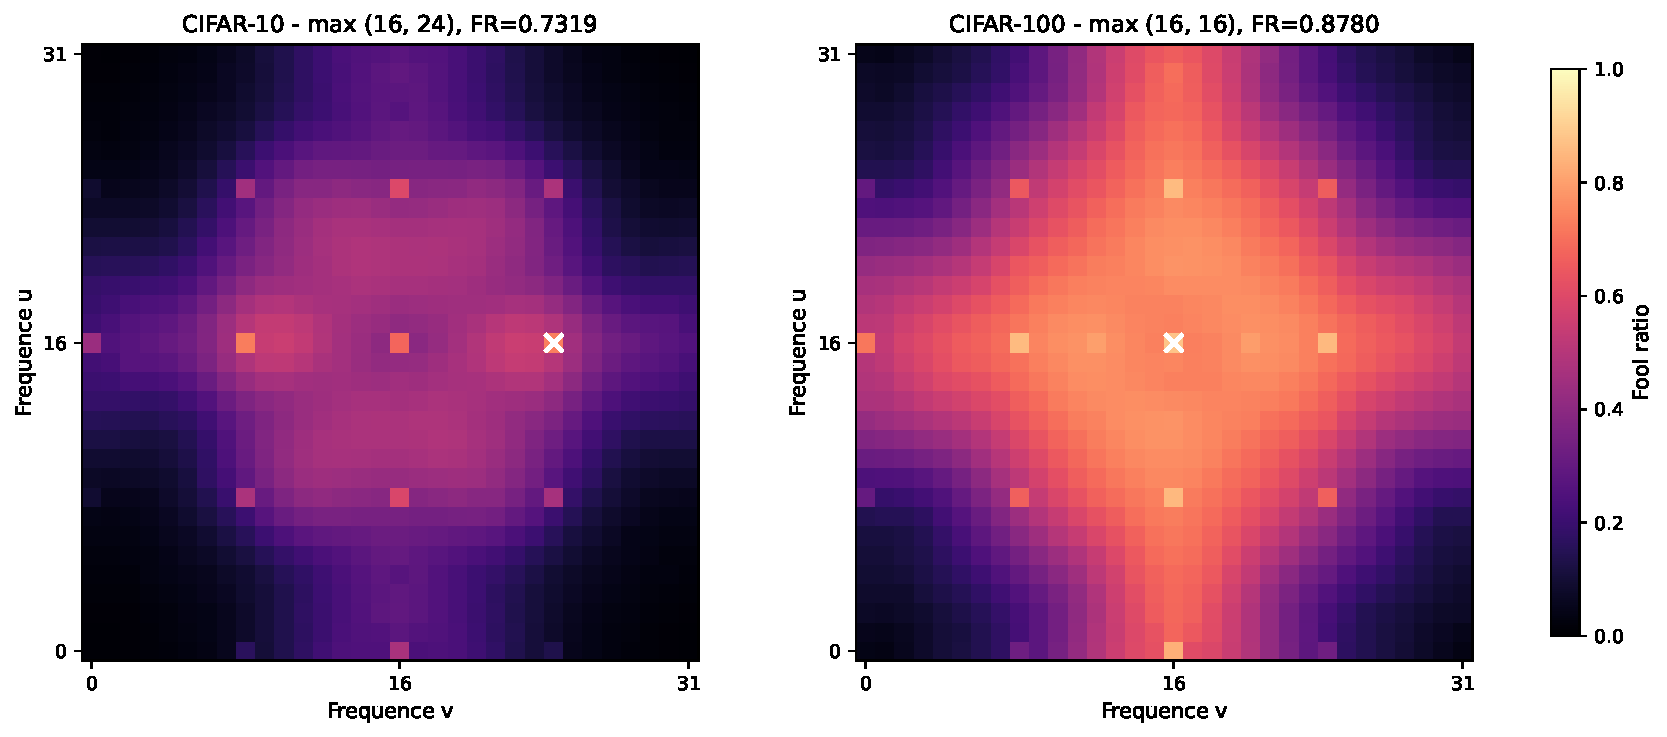
\includegraphics[width=0.7\textwidth]{figures/results/fourier_heatmap_comparison_vgg_cifar10_cifar100.pdf}
    \caption{Heatmaps de sensibilité fréquentielle pour \texttt{VGGSmallBN} sur CIFAR-10 et CIFAR-100.}
    \label{fig:heatmap_comparison_vgg_cifar10_cifar100}
\end{figure}
L'observation principale est que la sensibilité n'est pas uniforme dans le domaine de Fourier. Certaines
fréquences provoquent très peu de changements de prédiction, tandis que d'autres produisent un
\textit{fool ratio} beaucoup plus élevé.

Les deux heatmaps présentent une organisation structurée, avec des zones de forte sensibilité autour
de certaines lignes et intersections fréquentielles, notamment près des coordonnées liées à $16$. Cette
structure suggère que la vulnérabilité du modèle n'est pas un effet aléatoire, mais dépend de certaines
directions fréquentielles privilégiées.

Une comparaison descriptive avec le spectre moyen des images propres est donnée en
annexe~\ref{annexe:spectres_moyens_cifar}. Cette analyse vise a donne une autre manière d'interpréter
les résultats sous le prisme des statistiques fréquentielles des données brutes.

Pour compléter la lecture des heatmaps, la figure~\ref{fig:fool_ratio_histogram_comparison_vgg_cifar10_cifar100}
représente la distribution des \textit{fool ratios} sur les $32 \times 32 = 1024$ fréquences testées.

Sur CIFAR-10, la plupart des fréquences ont un effet faible ou modéré, et seules quelques directions
atteignent des \textit{fool ratios} élevés. La sensibilité du modèle est donc réelle, mais relativement
localisée dans le domaine fréquentiel.

\begin{figure}[H]
    \centering
    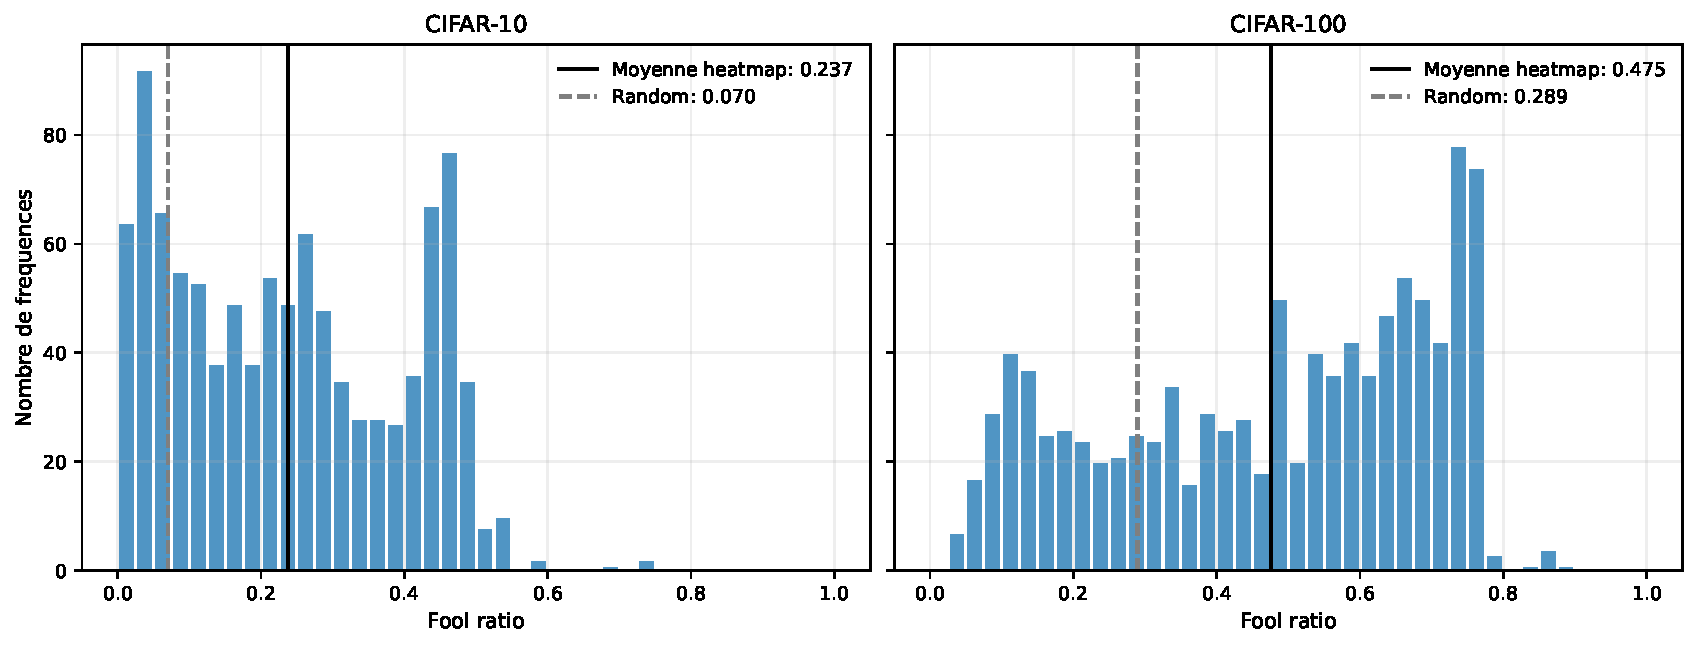
\includegraphics[width=0.9\textwidth]{figures/results/fourier_fool_ratio_histogram_comparison_vgg_cifar10_cifar100.pdf}
    \caption{Distribution des \textit{fool ratios} obtenus sur l'ensemble des fréquences de Fourier testées.}
    \label{fig:fool_ratio_histogram_comparison_vgg_cifar10_cifar100}
\end{figure}

Sur CIFAR-100, la distribution est déplacée vers la droite : la moyenne passe de $0.2375$ à $0.4755$.
Le modèle est donc globalement plus fragile, ce qui est cohérent avec la difficulté plus élevée de la
tâche discutée en annexe~\ref{annexe:marges-logits}. Cependant, cette fragilité reste structurée : toutes les fréquences ne produisent pas le même
effet, et certaines directions demeurent nettement plus perturbatrices que d'autres.

L'histogramme complète donc la lecture visuelle des heatmaps. Il montre que la sensibilité n'est pas
seulement non uniforme spatialement : elle est aussi très dispersée quantitativement. Une petite partie
des fréquences concentre l'essentiel de l'effet perturbateur.

\subsection{Fréquences les plus sensibles}
\label{subsec:frequences_plus_sensibles}

L'analyse des heatmaps permet d'identifier les fréquences les plus perturbatrices pour chaque
dataset. Le tableau~\ref{tab:frequences_plus_sensibles} présente les trois fréquences obtenant les
plus grands \textit{fool ratios}.

\begin{table}[H]
    \centering
    \begin{tabular}{c|cc|cc}
        & \multicolumn{2}{c|}{CIFAR-10} & \multicolumn{2}{c}{CIFAR-100} \\
        Rang & Fréquence $(u,v)$ & \textit{Fool ratio} & Fréquence $(u,v)$ & \textit{Fool ratio} \\
        \hline
        1 & $(16,24)$ & $0.7319$ & $(16,16)$ & $0.8780$ \\
        2 & $(16,8)$  & $0.7295$ & $(16,8)$  & $0.8585$ \\
        3 & $(16,16)$ & $0.6765$ & $(24,16)$ & $0.8565$ \\
    \end{tabular}
    \caption{Fréquences les plus sensibles pour \texttt{VGGSmallBN} sur CIFAR-10 et CIFAR-100.}
    \label{tab:frequences_plus_sensibles}
\end{table}

Les fréquences dominantes se concentrent autour d'une même famille de directions. Sur CIFAR-10, les deux premières fréquences,
$(16,24)$ et $(16,8)$, sont conjuguées modulo $32$ et obtiennent logiquement des \textit{fool ratios} presque
identiques. 

Sur CIFAR-100, la fréquence la plus sensible devient $(16,16)$, qui est sa propre conjuguée modulo
$32$.

\subsection{Stabilité des zones sensibles entre plusieurs entraînements}
\label{subsec:stabilite_multi_seeds}

Les heatmaps précédentes montrent que certaines fréquences sont beaucoup plus sensibles que
d'autres. Cependant, une question importante reste à vérifier : cette structure est-elle propre à un
entraînement particulier du modèle, ou reste-t-elle observable lorsque l'on change la seed
d'initialisation ?

\begin{figure}[H]
    \centering
    \vspace{-10pt} 

    \begin{minipage}{0.35\textwidth}
        \centering
        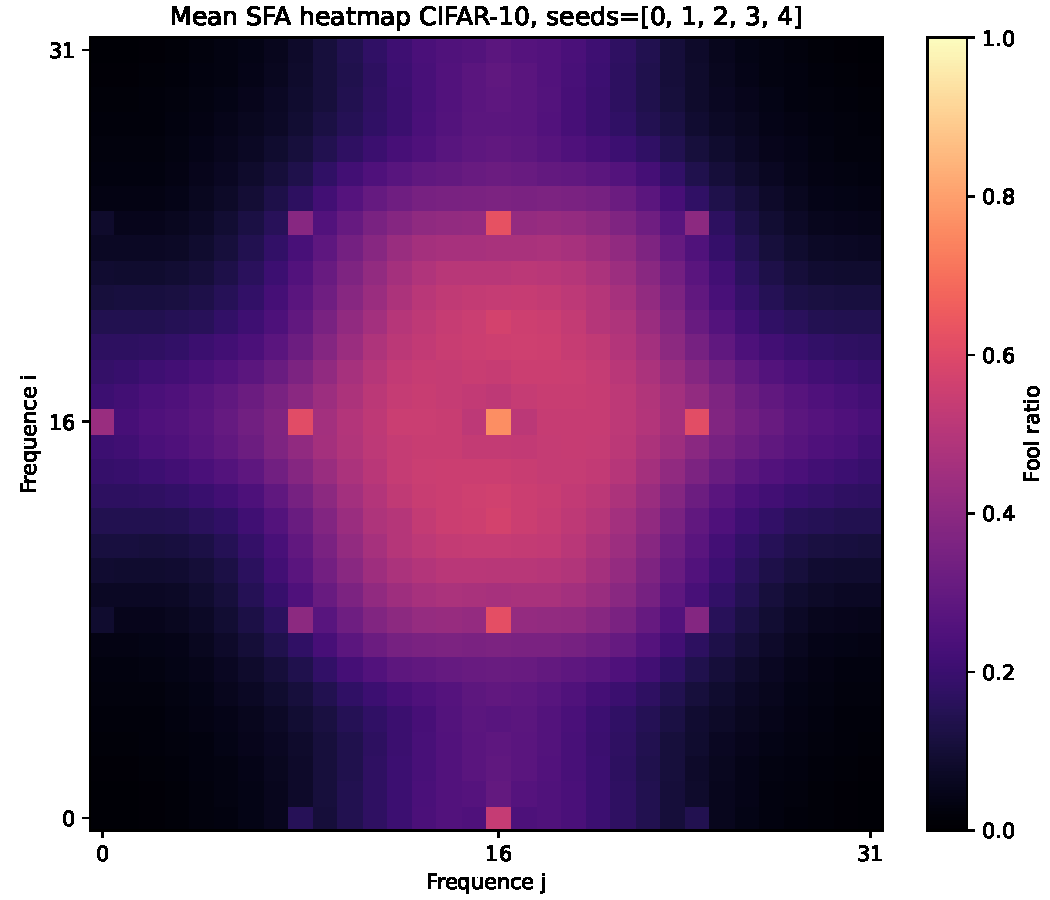
\includegraphics[width=\textwidth]{figures/results/stability_cifar10_heatmap_mean.pdf}
        \vspace{-5pt} 
        {\small (a) CIFAR-10 -- \textit{fool ratio} moyen}
    \end{minipage}
    \hspace{0.05\textwidth} 
    \begin{minipage}{0.35\textwidth}
        \centering
        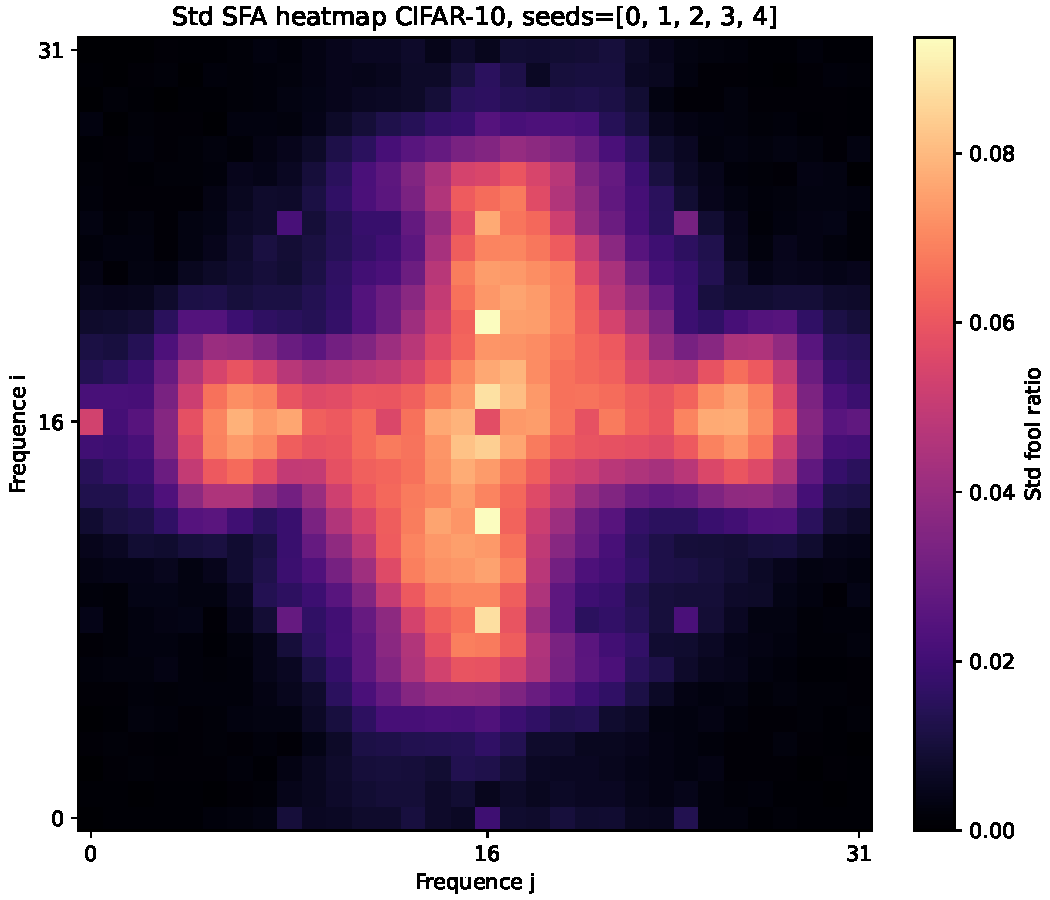
\includegraphics[width=\textwidth]{figures/results/stability_cifar10_heatmap_std.pdf}
        \vspace{-5pt}
        {\small (b) CIFAR-10 -- écart-type}
    \end{minipage}

    \vspace{2pt} 

    \begin{minipage}{0.35\textwidth}
        \centering
        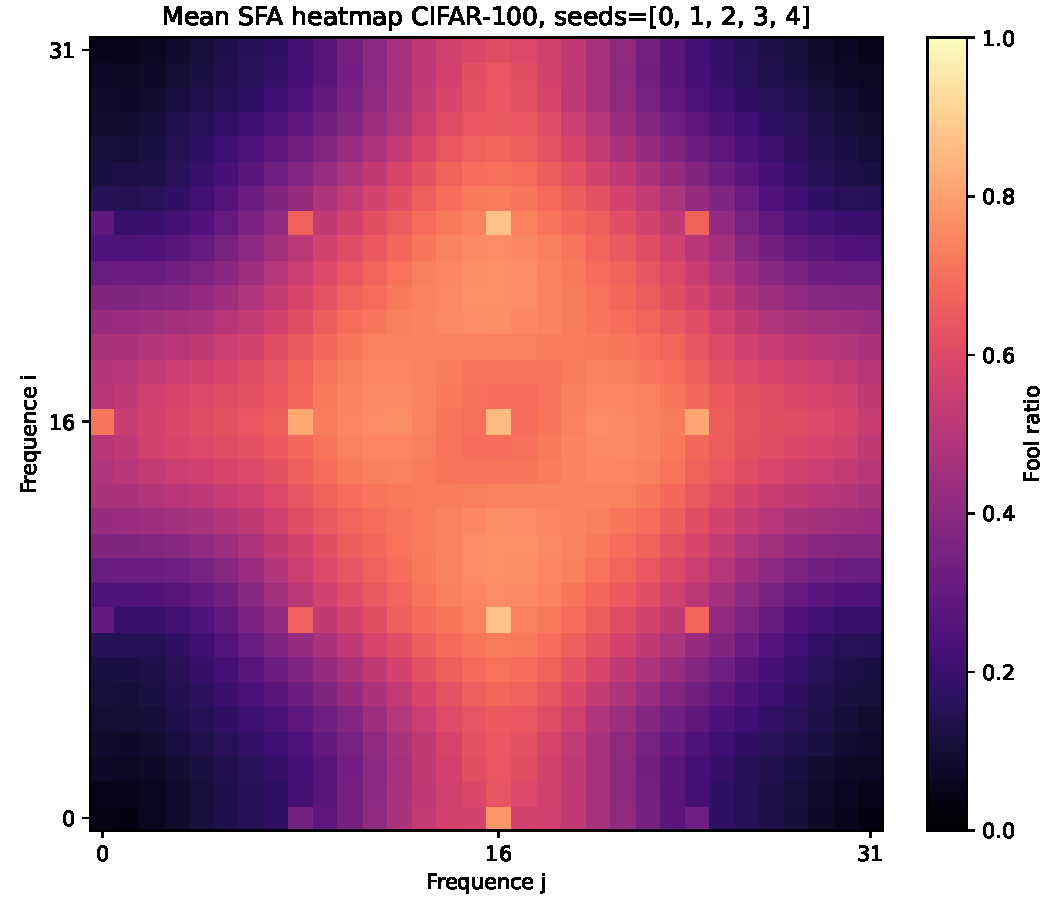
\includegraphics[width=\textwidth]{figures/results/stability_cifar100_heatmap_mean.pdf}
        \vspace{-5pt}
        {\small (c) CIFAR-100 -- \textit{fool ratio} moyen}
    \end{minipage}
    \hspace{0.05\textwidth}
    \begin{minipage}{0.35\textwidth}
        \centering
        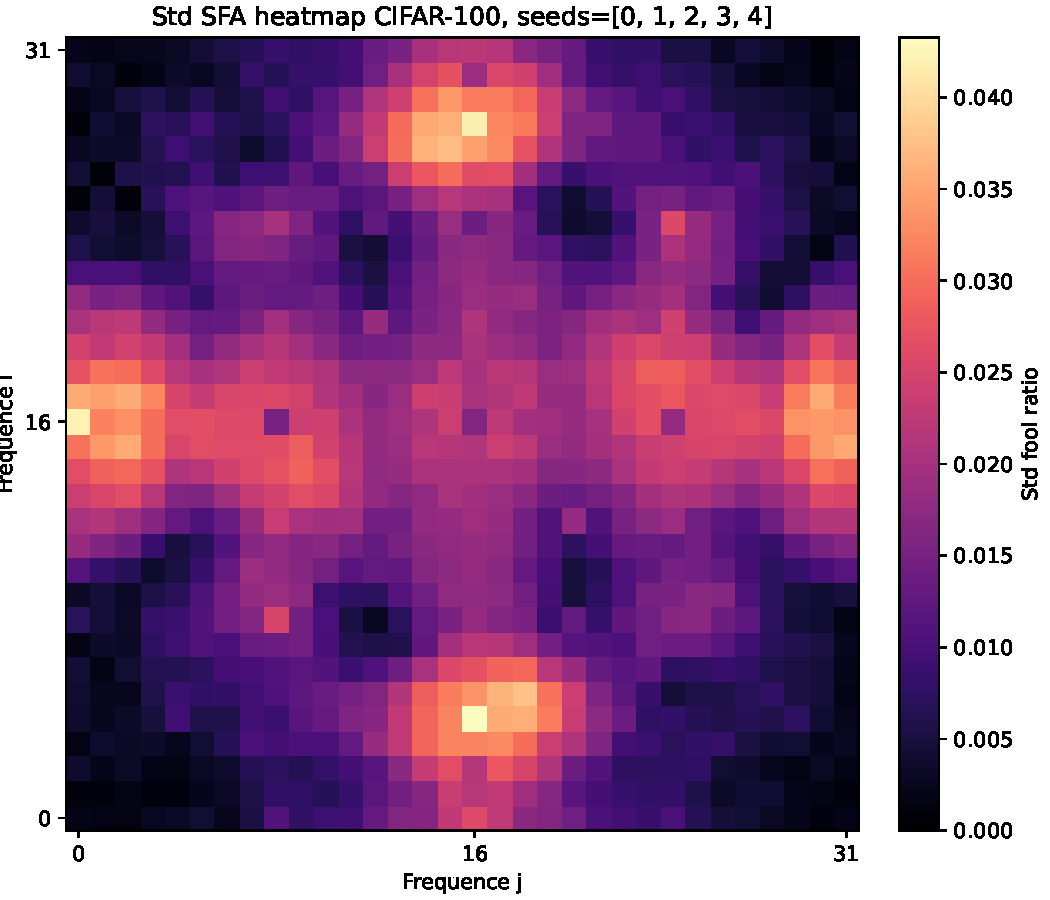
\includegraphics[width=\textwidth]{figures/results/stability_cifar100_heatmap_std.pdf}
        \vspace{-5pt}
        {\small (d) CIFAR-100 -- écart-type}
    \end{minipage}

    \caption{Stabilité de la sensibilité fréquentielle de \texttt{VGGSmallBN} sur CIFAR-10 et CIFAR-100.}
    \label{fig:stability_cifar10_cifar100_mean_std}
\end{figure}

Pour répondre à cette question, nous avons répété l'expérience sur CIFAR-10 et CIFAR-100 avec cinq
entraînements indépendants de \texttt{VGGSmallBN}. Le protocole d'entraînement est conservé identique
pour chaque run. Seule la seed est modifiée.

La figure~\ref{fig:stability_cifar10_cifar100_mean_std} présente,
pour chaque dataset, la heatmap moyenne obtenue sur les cinq seeds ainsi que l'écart-type associé
à chaque fréquence.

Les résultats montrent que la structure globale des heatmaps reste très stable entre les entraînements.
Sur CIFAR-10, les zones de forte sensibilité restent localisées autour des mêmes régions fréquentielles,
en particulier autour des fréquences médianes liées aux axes centraux. Sur CIFAR-100, cette structure
est encore plus marquée : une large zone de forte sensibilité apparaît autour des fréquences centrales.

% Cette stabilité est confirmée quantitativement par les corrélations entre heatmaps. Sur CIFAR-10, la
% corrélation de Pearson moyenne entre heatmaps est d'environ $0.976$, et la corrélation de Spearman
% moyenne d'environ $0.985$. Sur CIFAR-100, ces valeurs montent respectivement à environ $0.994$
% et $0.992$. Les heatmaps sont donc très proches d'un entraînement à l'autre, aussi bien en valeur
% qu'en classement relatif des fréquences.

Le tableau~\ref{tab:stability_multiseed_metrics} résume les principales métriques moyennées sur les cinq
seeds. L'accuracy propre reste proche de celle du modèle principal, tandis que l'accuracy après attaque
diminue fortement. Cela montre que le \textit{fool ratio} élevé correspond bien à une dégradation réelle
des performances du modèle, et pas seulement à des changements de prédiction sans conséquence sur
la classification correcte.

\begin{table}[H]
    \centering
    \begin{tabular}{l|c|c}
        \hline
        Métrique & CIFAR-10 & CIFAR-100 \\
        \hline
        Accuracy propre moyenne & $93.08\,\%$ & $72.50\,\%$ \\
        Meilleur \textit{fool ratio} moyen & $76.35\,\%$ & $87.64\,\%$ \\
        Accuracy après attaque moyenne & $23.39\,\%$ & $11.83\,\%$ \\
        Taux de succès sur images initialement correctes & $76.38\,\%$ & $85.18\,\%$ \\
        % Corrélation de Pearson moyenne entre heatmaps & $0.976$ & $0.994$ \\
        % Corrélation de Spearman moyenne entre heatmaps & $0.985$ & $0.992$ \\
        \hline
    \end{tabular}
    \caption{Résumé de l'expérience de stabilité multi-seeds sur CIFAR-10 et CIFAR-100.}
    \label{tab:stability_multiseed_metrics}
\end{table}

\subsection{Amplification interne des fréquences sensibles}
\label{subsec:amplification_interne_sfa}

Les heatmaps précédentes montrent que certaines fréquences de Fourier produisent des \textit{fool ratios}
nettement plus élevés que d'autres. Pour mieux comprendre ce phénomène, nous avons analysé la manière
dont ces perturbations se propagent à l'intérieur du réseau.

Pour une perturbation \(\delta\), nous notons \(G_l(\delta)\) l'amplification normalisée mesurée à la
couche \(l\). Cette quantité compare la norme moyenne de la variation d'activation provoquée par la
perturbation à la norme de la perturbation d'entrée. Elle permet donc de comparer l'effet relatif de
différentes fréquences dans les blocs internes du réseau et au niveau des logits.

Afin de rendre cette analyse plus robuste, nous l'avons répétée sur les cinq checkpoints utilisés dans
l'expérience de stabilité multi-seeds. Les fréquences sont regroupées à partir de la heatmap moyenne :
les \(50\) fréquences les plus sensibles, \(50\) fréquences de sensibilité intermédiaire, et les \(50\)
fréquences les moins sensibles. La fréquence principale correspond à la meilleure fréquence moyenne
sur les cinq seeds.

\begin{figure}[H]
    \centering
    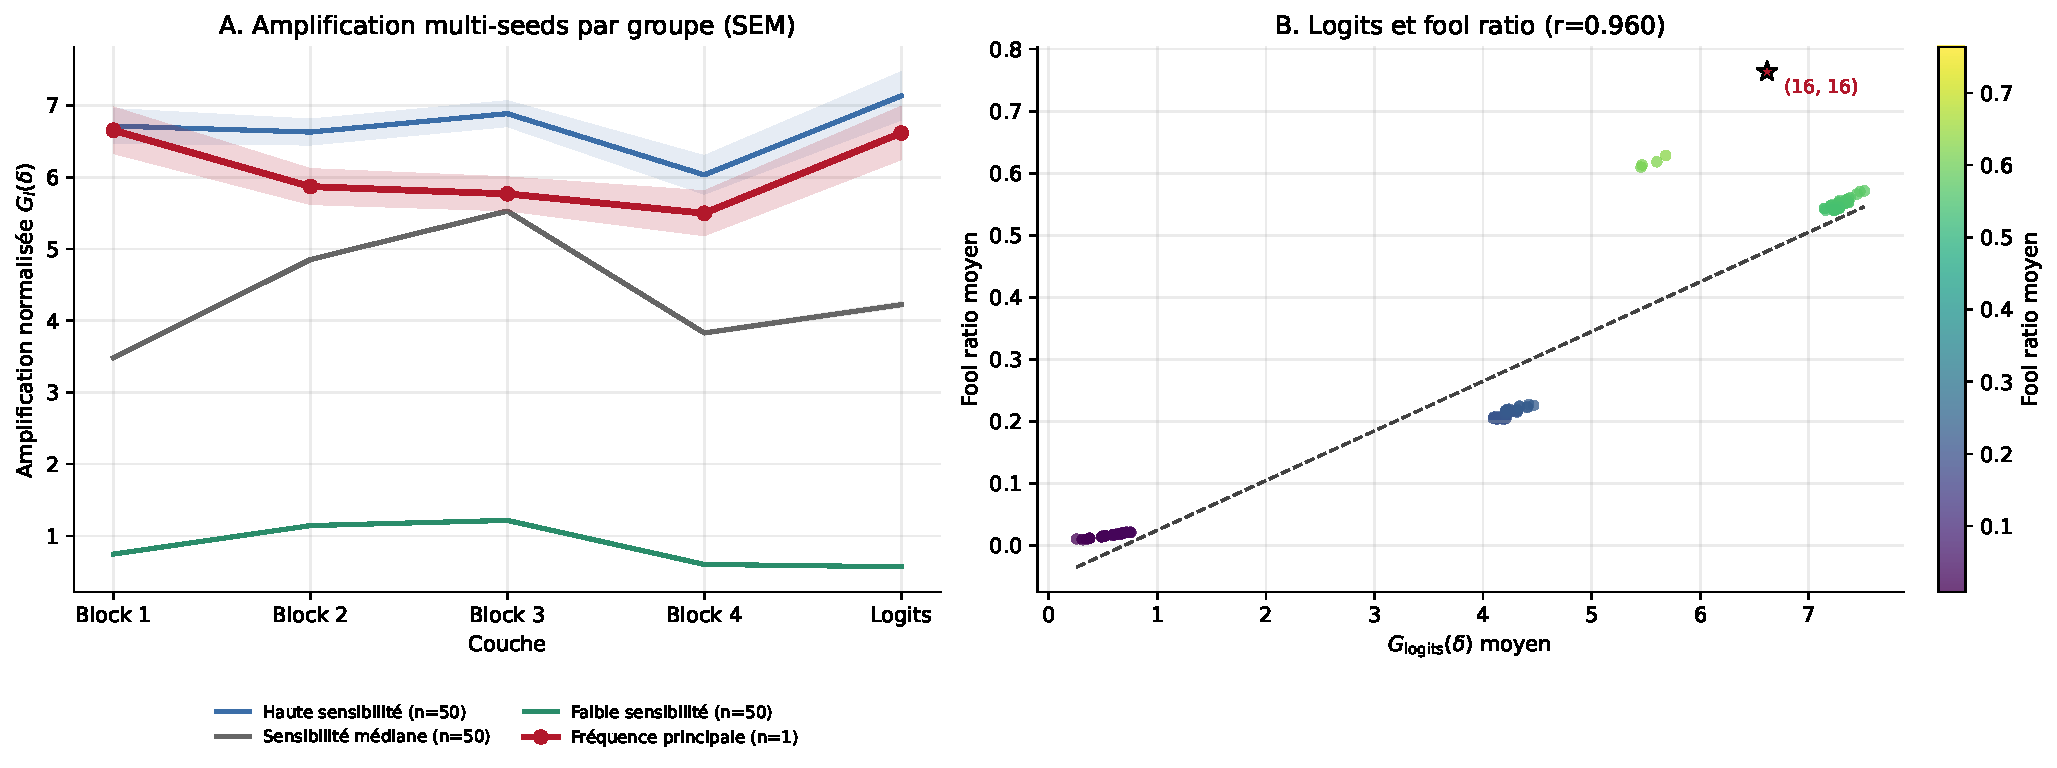
\includegraphics[width=\textwidth]{figures/results/layerwise_frequency_sensitivity_analysis_vgg_cifar10_multiseed.pdf}
    \caption{Analyse multi-seeds de l'amplification interne des perturbations de Fourier dans
    \texttt{VGGSmallBN} sur CIFAR-10. À gauche, les fréquences sont regroupées selon leur
    \textit{fool ratio} moyen. Les bandes indiquent l'erreur standard sur les cinq seeds. À droite,
    l'amplification moyenne au niveau des logits est comparée au \textit{fool ratio} moyen.}
    \label{fig:layerwise_frequency_sensitivity_multiseed}
\end{figure}

La figure~\ref{fig:layerwise_frequency_sensitivity_multiseed} montre que logiquement les fréquences les plus
sensibles sont aussi celles qui produisent les amplifications internes les plus élevées. 

Le panneau de droite montre une corrélation élevée entre l'amplification moyenne au niveau des logits
et le \textit{fool ratio} moyen. Cela suggère que la sensibilité finale du modèle n'est pas seulement liée
au couple $(u, v)$ choisi, mais aussi à la manière dont cette perturbation est propagée et
amplifiée par le réseau.

Cette observation fait le lien avec le cadre théorique et avec l'interprétation locale introduite au
chapitre précédent : même si le réseau réel n'est pas globalement linéaire, certaines directions
fréquentielles semblent être davantage amplifiées par son comportement local, ce qui peut expliquer
leur effet plus important sur les prédictions.

Une visualisation plus détaillée des heatmaps internes par couche est donnée en annexe~\ref{annexe:heatmaps_internes_couches}.

\subsection{Comparaison avec un bruit aléatoire}
\label{subsec:comparaison_bruit_aleatoire}

Pour vérifier que les fortes valeurs obtenues par la SFA ne proviennent pas uniquement de l'amplitude
de la perturbation, nous comparons la meilleure direction de Fourier avec une baseline de bruit
aléatoire. Dans cette baseline, chaque pixel est perturbé indépendamment par un bruit uniforme
borné dans le même intervalle d'amplitude. La contrainte est donc la même que pour la SFA :
\[
    \|\delta\|_{\infty} \leq \epsilon,
    \qquad
    \epsilon = 10/255.
\]
La différence vient de la structure de la perturbation : la SFA utilise un motif fréquentiel cohérent,
tandis que la baseline aléatoire ne privilégie aucune direction particulière.

\textbf{A FAIRE : }
Il faudrais s'assurer que  $\|\delta_{SFA}\|_{2} = \|\delta_{random}\|_{2}$

La figure~\ref{fig:sfa_vs_random_comparison_vgg_cifar10_cifar100} compare, pour chaque dataset,
le \textit{fool ratio} de la meilleure fréquence SFA avec le \textit{fool ratio} moyen obtenu par bruit
aléatoire.

\begin{figure}[H]
    \centering
    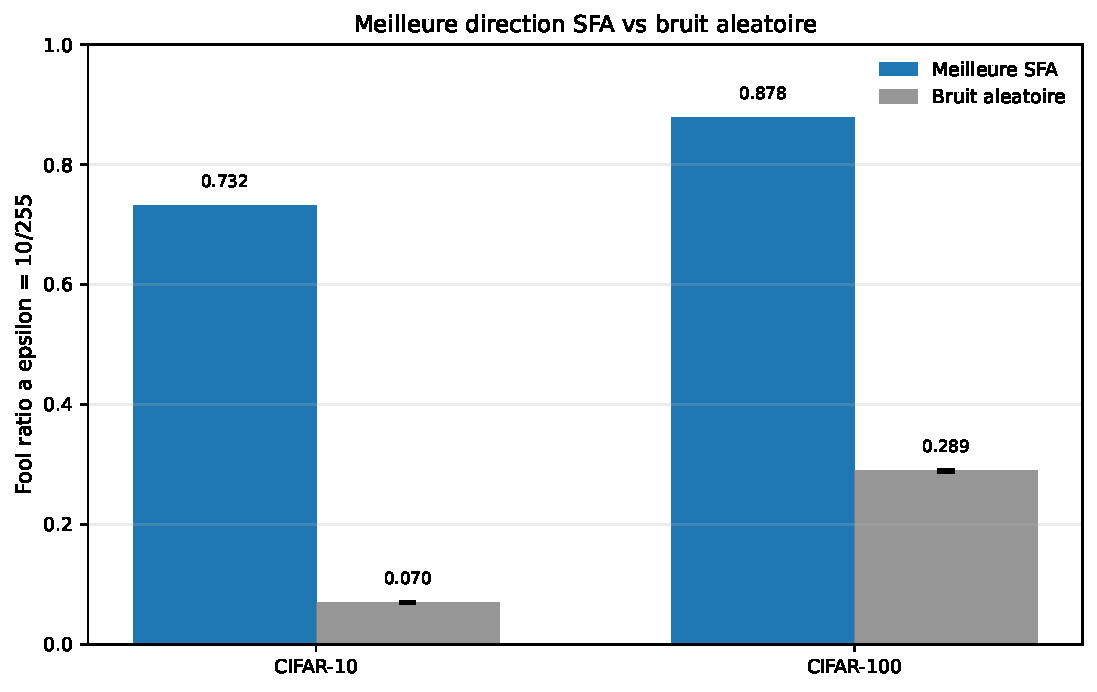
\includegraphics[width=0.85\textwidth]{figures/results/sfa_vs_random_comparison_vgg_cifar10_cifar100.pdf}
    \caption{Comparaison entre la meilleure direction SFA et un bruit aléatoire uniforme de même amplitude
    $\epsilon = 10/255$. Pour le bruit aléatoire, la barre d'erreur représente l'écart-type sur 100 essais.}
    \label{fig:sfa_vs_random_comparison_vgg_cifar10_cifar100}
\end{figure}

Sur CIFAR-10, la différence est très nette : la meilleure direction de Fourier atteint un
\textit{fool ratio} de $0.7319$, alors que le bruit aléatoire moyen atteint seulement $0.0704$.
La perturbation de Fourier est donc environ dix fois plus efficace qu'un bruit aléatoire de même
amplitude. Ce résultat indique que la vulnérabilité observée ne peut pas être expliquée par la seule
taille de la perturbation.

Sur CIFAR-100, le bruit aléatoire est déjà plus perturbateur, avec un \textit{fool ratio} moyen de
$0.2892$. Confirment que le modèle entraîné sur CIFAR-100 est globalement plus fragile. Cependant,
la meilleure direction SFA atteint $0.8780$, soit environ trois fois le niveau du bruit aléatoire moyen.

\subsection{Effet de l'amplitude de la perturbation}
\label{subsec:effet_amplitude_epsilon}

Jusqu'ici, les résultats principaux ont été obtenus avec $\epsilon = 10/255$. Cette valeur permet de
comparer nos résultats au protocole original, mais elle peut produire des motifs visibles sur des images
de très faible résolution. Or une attaque adversariale a pour but de rester
peu perceptible pour l'humain. Nous testons donc si les fréquences les plus sensibles conservent un effet pour des
valeurs plus faibles de $\epsilon$.

Pour cela, nous fixons la fréquence la plus sensible de chaque dataset, puis nous faisons varier
$\epsilon$ dans l'ensemble suivant :
\[
    \epsilon \in
    \left\{
        \frac{1}{255},
        \frac{2}{255},
        \frac{3}{255},
        \frac{5}{255},
        \frac{10}{255}
    \right\}.
\]

\begin{figure}[H]
    \centering
    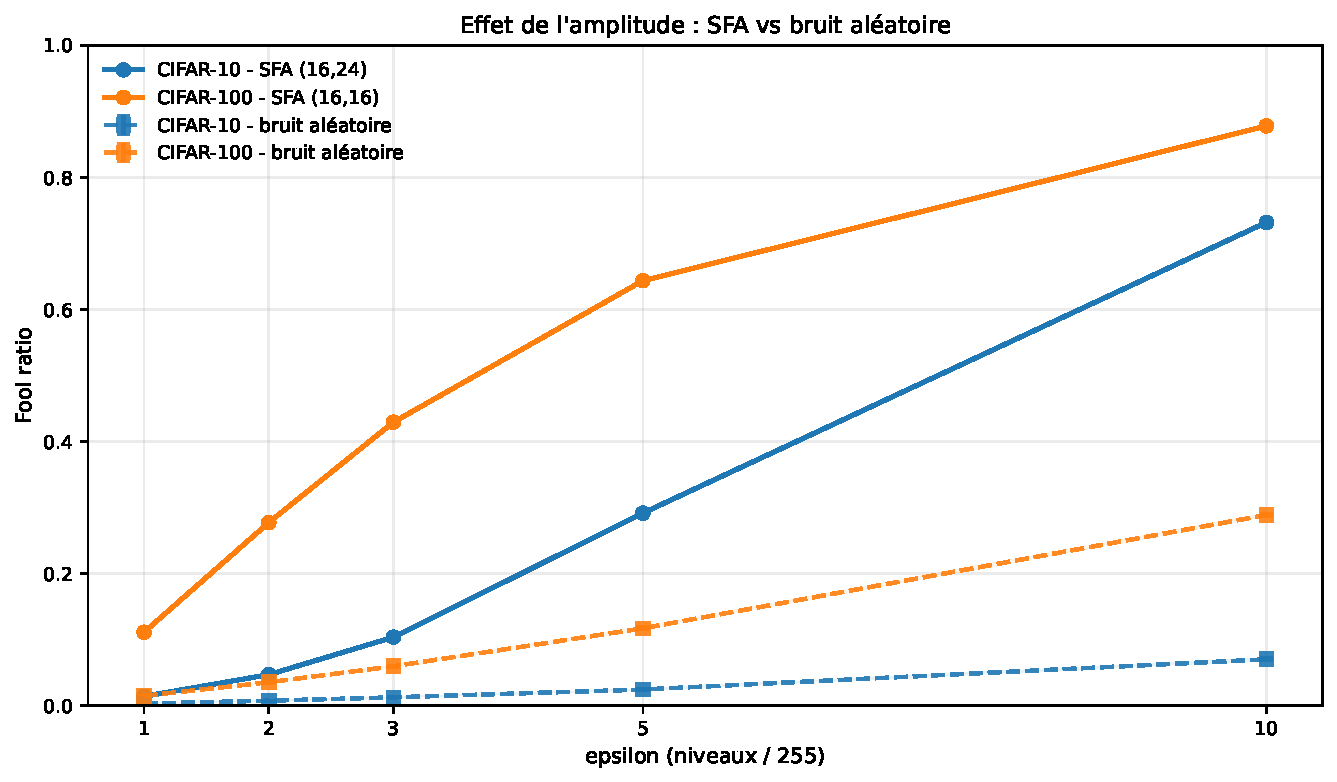
\includegraphics[width=0.55\textwidth]{figures/results/sfa_epsilon_sweep_with_random_comparison_vgg_cifar10_cifar100.pdf}
    \caption{Évolution du \textit{fool ratio} en fonction de l'amplitude $\epsilon$ pour la meilleure fréquence
    SFA de chaque dataset.}
    \label{fig:sfa_epsilon_sweep_comparison_vgg_cifar10_cifar100}
\end{figure}

La figure~\ref{fig:sfa_epsilon_sweep_comparison_vgg_cifar10_cifar100} montre une augmentation
régulière du \textit{fool ratio} lorsque $\epsilon$ augmente. Ce comportement est attendu : plus la
perturbation est grande, plus elle modifie l'image d'entrée, et plus elle a de chances de déplacer la
prédiction du modèle. Mais elle confirme aussi que dans ce contexte, l'amplitude de la perturbation 
est un facteur important de l'efficacité de l'attaque, nous obligeant rendre la perturbation plus moins
discrète pour obtenir un effet plus significatif.

\begin{figure}[H]
    \centering
    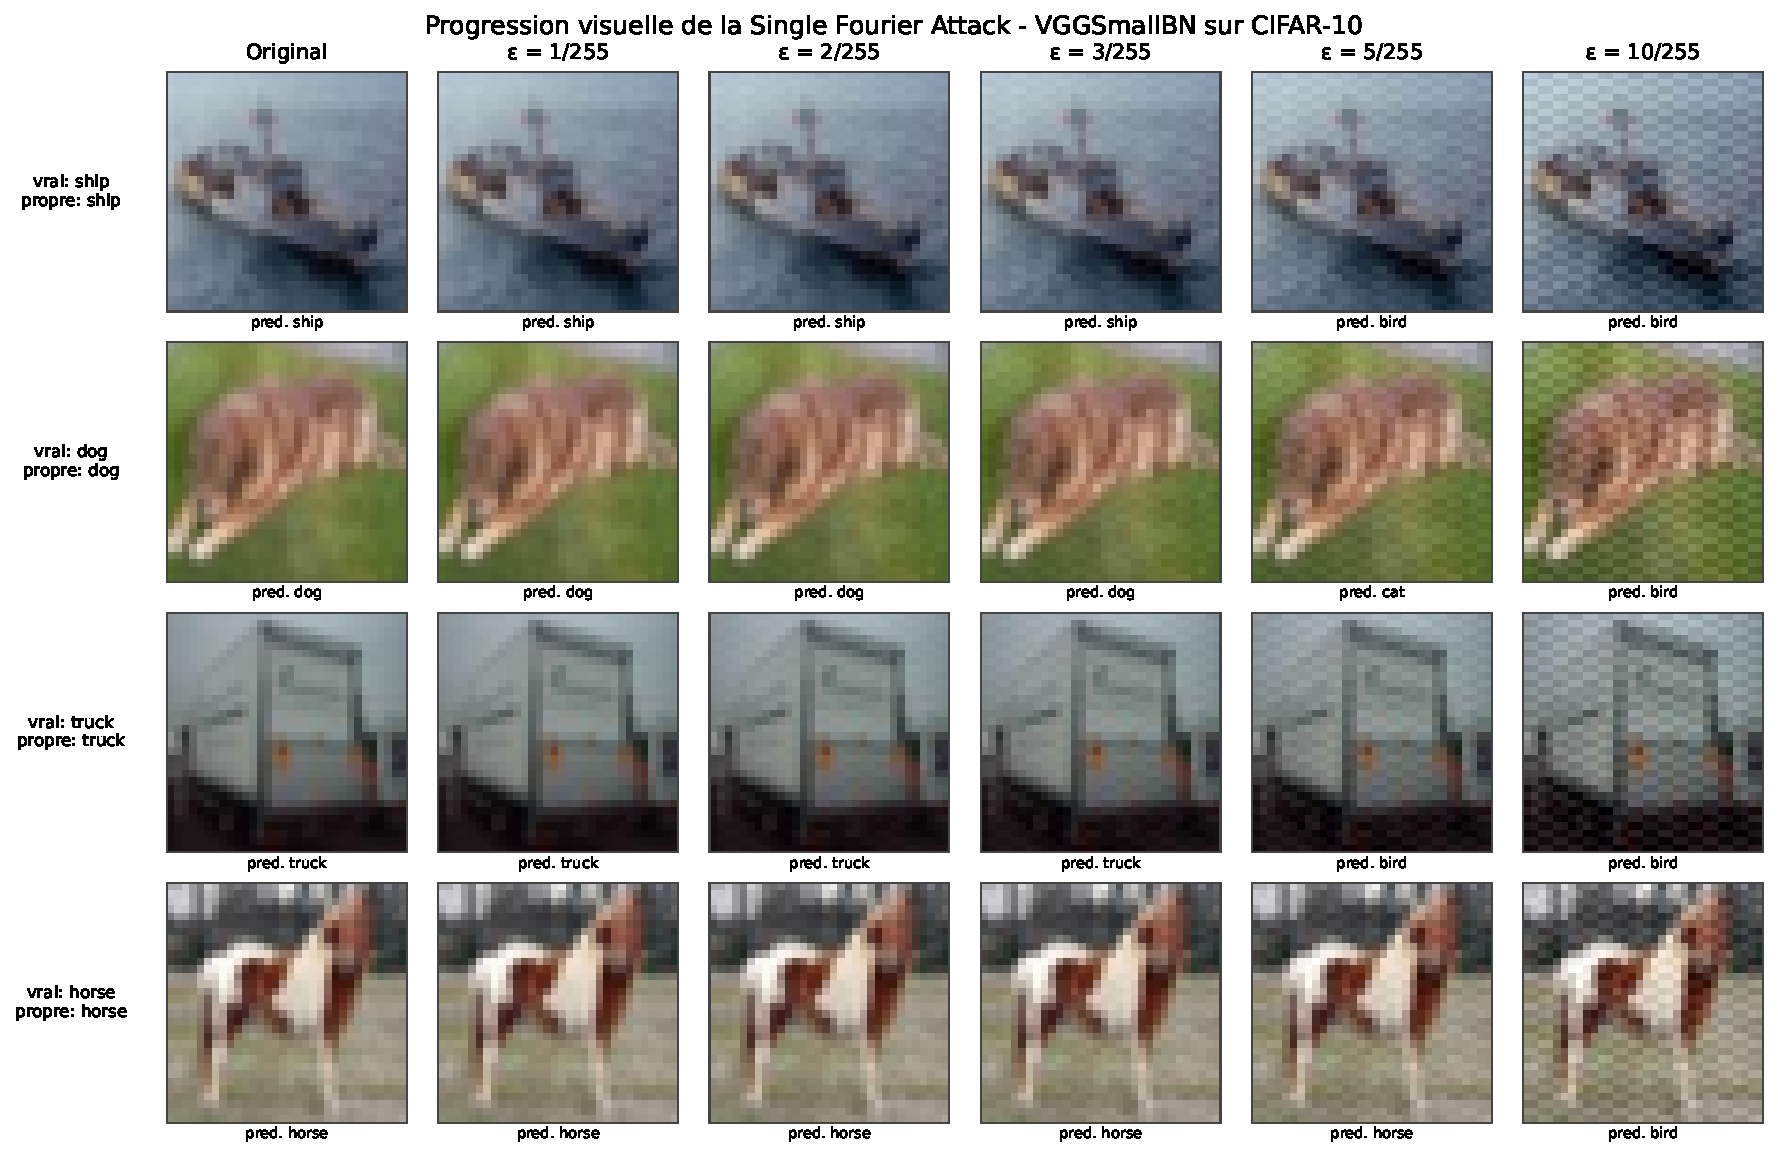
\includegraphics[width=1\textwidth]{figures/results/sfa_visual_progression_vgg_cifar10.pdf}
    \caption{Progression visuelle d'une attaque \textit{Single Fourier Attack} sur des images de CIFAR-10.}
    \label{fig:sfa_visual_progression_vgg_cifar10}
\end{figure}

Comme l'illustre la figure~\ref{fig:sfa_visual_progression_vgg_cifar10}, l'augmentation de l'amplitude rend le motif de 
Fourier de plus en plus intrusif. On remarque notamment qu'à partir d'une valeur de $\epsilon = 3/255$, la perturbation 
structurée en forme de grille commence à être distinctement visible à l'oeil nu. 

Il convient néanmoins de nuancer ces observations. Les expériences sont réalisées sur des images de
très basse résolution ($32\times32$ pixels) et avec une architecture volontairement restreinte
(\texttt{VGGSmallBN}). Les conclusions ne doivent donc pas être généralisées directement à des images
de haute résolution ou à des architectures beaucoup plus profondes. Elles montrent cependant que,
dans notre cadre expérimental, l'effet des perturbations de Fourier dépend fortement de l'amplitude.

\subsection{Lien avec le cadre théorique}
\label{subsec:discussion_lien_cadre_theorique}

Les résultats expérimentaux obtenus dans ce chapitre permettent de revenir au cadre théorique
développé au chapitre précédent. Dans le modèle linéaire idéalisé, les fonctions de Fourier apparaissent
comme des directions privilégiées des opérateurs de convolution. Dans un CNN réel, cette propriété
ne s'applique plus directement au réseau complet, mais elle peut rester pertinente localement à travers
le jacobien du modèle.

Les heatmaps obtenues expérimentalement vont dans ce sens. Si toutes les directions fréquentielles
étaient équivalentes pour le modèle, les cartes de sensibilité seraient beaucoup plus uniformes. Or ce
n'est pas ce que l'on observe : certaines fréquences produisent des \textit{fool ratios} nettement plus
élevés que d'autres, alors que toutes les perturbations respectent la même contrainte $\ell_\infty$.

La stabilité multi-seeds renforce cette interprétation. Les zones sensibles ne semblent pas dépendre
uniquement d'une initialisation particulière du réseau : elles restent visibles lorsque l'entraînement est
répété avec différentes seeds. La comparaison avec le bruit aléatoire montre également que l'effet ne
provient pas seulement de l'amplitude de la perturbation, mais de sa structure fréquentielle.

Ces résultats montrent que l'intuition issue du cadre théorique reste
observable expérimentalement pour \texttt{VGGSmallBN} : certaines directions de Fourier sont plus perturbatrices que d'autres,
ce qui est compatible avec une amplification locale de ces directions dans le réseau.

\paragraph{Influence du mélange entre canaux.}

Precedement nous avions considéré qu'une direction sensible peut aussi faire intervenir un mélange entre
les canaux couleur, sous la forme $a \otimes \varphi_{u,v}$. Le protocole principal utilise une version simplifiée de
cette idée : le même motif de Fourier est appliqué aux trois canaux, ce qui correspond à une direction
couleur de type $(1,1,1)$.

Une analyse complémentaire de cette simplification est proposée en annexe~\ref{annexe:color_sfa}.
Elle vise à montrer que le choix du mélange entre canaux est negligeable en comparaison du choix de maximiser l'amplification de l'attaque.

\section{Synthèse du chapitre}
\label{sec:synthese_chapitre4}

Les expériences réalisées confirment que la sensibilité de \texttt{VGGSmallBN} aux perturbations de
Fourier est fortement non uniforme. Sur CIFAR-10 comme sur CIFAR-100, certaines fréquences
provoquent beaucoup plus de changements de prédiction que d'autres, alors que toutes les perturbations
respectent la même contrainte $\ell_\infty$.

Cette structure reste stable entre plusieurs entraînements indépendants et dépasse nettement l'effet
obtenu avec un bruit aléatoire de même amplitude. Le balayage de $\epsilon$ montre toutefois que
l'efficacité de l'attaque dépend fortement de l'amplitude, en particulier sur des images de basse
résolution comme celles de CIFAR.

Enfin, l'analyse interne suggère que les fréquences les plus sensibles sont aussi celles qui sont le plus
amplifiées dans les représentations du réseau. Ces observations ne prouvent pas que le modèle réel se
comporte comme un opérateur linéaire global, mais elles montrent que la structure fréquentielle mise
en évidence dans le cadre théorique reste partiellement visible dans le comportement local du modèle.
